
% this file is called up by thesis.tex
% content in this file will be fed into the main document

%: ----------------------- introduction file header -----------------------
\begin{savequote}[50mm]
Buscar cita nueva
\end{savequote}


\newcommand{\pathchapsix}{6_implementation}
\newcommand{\codigo}[1]{``\texttt{#1}''}


\chapter{Implementation}
\label{cha:implementation}

% the code below specifies where the figures are stored
\ifpdf
    \graphicspath{{\pathchapsix/figures/PNG/}{\pathchapsix/figures/PDF/}{\pathchapsix/figures/}}
\else
    \graphicspath{{\pathchapsix/figures/EPS/}{\pathchapsix/figures/}}
\fi


%------------------------------------------------------------------------- 

% INTRO:
% implementación de las ideas vistas con anterioridad
% TODO igual estaría bien meterlo antes de la sección 4, dado que se usa en su evaluación datos de aquí

%%\section{Introduction}

% Originally, the Internet was basically composed of a small number of computers that were physically connected to a wired network.
% Over the years, the popularity of the Internet grew and connecting computers became easier and cheaper.
% Thanks to wireless technologies, devices can connect to the Internet without having to be connected to a network.
% 
% Nowadays, everyday objects like cars or washing machines start to be connected to the Internet to exchange information.
% This is what is currently known as the \emph{Internet of Things (IoT)} \citep{atzori_internet_2010}.
% We can organize the IoT into \emph{Spaces} or islands which cover a particular knowledge as proposed by \citet{abdulrazakCGF10}.
% Using Spaces, we can ease the creation of different \emph{Ambient Intelligence (AmI)} environments.
% For example, we can create a Space for our home where we connect our devices to form an AmI environment.
% Thus, the washing machine could plan to finish washing the clothes two minutes before the car gets home.

Integrating mobile or embedded devices is not trivial as they usually communicate using different protocols.
To solve this problem, the \acl{wot} initiative proposes to use well-established web standards to ease their communication.
However, the format of the data they exchange is also multifarious and application domain dependent.
This implies that data will not be meaningful in other domains unless a specialized system converts and reinterprets them.
A way to solve this problem is annotating the data semantically as proposed by the \ac{www} \citep{ChuaG10,kimKC11}.

Adding semantics to the \ac{iot} works well for devices with high computational capacity but it adds too much overhead for most of the devices composing the \ac{iot}.
To reduce this overhead in such devices, part of this computation is usually delegated to intermediaries \citep{honkola_smart-m3_2010}.
This approach reduces the overhead of semantically annotated data but brings other problems.
(1) When devices rely on others to provide information, it is not guarantee that the information accessed will accurately represent the last information available in the data providers (e.g., the sensors).
(2) Once we rely on those intermediaries, it is required that they are available at all time.
Otherwise, the devices would not be able to talk to each other.

We propose a solution where we use intermediaries to release some workload from the less powerful devices, but at the same time, we promote the direct communication between the devices.
In particular, our system uses intermediaries to search where the data is located in the \Space{} and queries the final devices directly.

In our solution, the devices can become or stop being intermediaries dynamically.
To decide which device will be an intermediary, we evaluate the state of a device (i.e., energy and computation capacity).
Using this dynamic architecture, the absence of a particular intermediary does not collapse the system.
In addition, our system is flexible enough to support a wide range of scenarios.

To enable the search for information in this system, intermediaries need to know the information available in the \Space{}.
To do that, they aggregate summaries sent by each device.
We propose alternatives to summarize and to aggregate this information taking into account the payload of the shared information and the accuracy of the search.

We compare our approach against other common approaches.
In particular, we focus on the energy aspect, demonstrating that our approach helps energy constrained devices to face fewer unnecessary requests.
We also evaluate other important metrics like the number of messages a device has to exchange to perform a request, and the accuracy of the search results provided by the intermediaries.
We perform this evaluation under different scenarios to prove the flexibility of our proposal.

In summary, we make the following contributions:
\begin{itemize}
\item We present a new architecture for managing semantics on the \ac{wot} which reduces the load for resource-constrained devices.
\item We propose and evaluate different approaches to aggregate and summarize the semantic information available in the \Space{} and enable semantic search in this architecture.
\item We demonstrate the advantages of our approach compared to other typical searching approaches under different scenarios.
\end{itemize}

The remainder of this chapter is organized as follows:
Section~\ref{background} discusses the related work.
Section~\ref{proposal} presents in detail our energy-aware architecture.
Section~\ref{sec:clues} describes the information that devices exchange to maintain this architecture.
Section~\ref{environment} presents our experimental environment and Section~\ref{results} evaluates our solution.
Finally, Section~\ref{conclusion} states the conclusions of our work.
%% SECCIÓN: CUÁL ES EL DISEÑO GENERAL QUE SE PODRÍA UTILIZAR DESDE FUERA Y QUE HA MOTIVADO NUESTRA IMPLEMENTACIÓN
\section{Designing Triple Spaces over a canonical RESTful interface}
% ALGO QUE DIGA QUE NO DEPENDE DE OTSOPACK
% TODO: other name? ``defined layers'' o así? cómo decir ``mira, lo importante es que puede haber diferentes grados de
% implementación aquí gracias al diseño que mostramos en esta sección en 5 palabras???

So far, the compatibility of Triple Spaces with the HTTP RESTful style has been proved both from a formal \cite{hernandez_formal_2010} and qualitative point of view \cite{gomez-goiri_complementarity_2011}.
In this section our model towards the achievement of this mapping will be discussed in detail.

\subsection{TSC resources}

As was previously stated, our RESTful API is based on the Triple Space Computing paradigm, which is a Tuplespace variation where the information is stored in RDF.
Three key concepts are important at this point: agents share information in a common \textbf{space}.
A space is identified by an URI.
Therefore, all the operations performed in Triple Space are performed against a particular space.
By default, all applications should connect to a common standard space, but they can optionally choose to connect to a particular private space.
Within a space, the information is stored in sets of \textbf{triples} called \textbf{graphs}.
Each graph can also be identified by an URI. The RDF \textbf{triples} are the underlying concept of all the Semantic Web languages.
Each triple is composed by a subject (which is a URI), a predicate (also a URI) and a value (which can be a URI or a literal), as shown in the Figure \ref{fig:ontology}.

As detailed later, the operations supported by Otsopack attempt to add or remove graphs, as well as to query for graphs or query for sets of triples retrieved from different graphs.
In order to perform the queries, which enable the selection of a subset of the semantic content hold in a given space, a \textbf{template} is required.
Although more sophisticated query languages like SPARQL exist, in Otsopack wildcard templates are used, which are special triples with optional wildcard subject, predicate and/or objects.
For example, the template \texttt{?s foaf:knows kth:sven} could be employed to select instances which represent people who know Sven (see Figure \ref{fig:ontology}).


\InsertFig{semanticExample}{fig:ontology}{
  Semantic example
}{
  Sample triples expressed both grafically and in the RDF triple form.
  At the bottom a template example is shown.
  Aliases for the beginning of most URIs, known as prefixes in most Semantic languages, are used for the lack of clarity.
}{1}{}


\subsection{Adopted TSC primitives}
\label{sec:primitives}

TSC derives some primitives originally defined in the Linda language \cite{gelernter_generative_1985} to access to the semantic information hold in each graph.
In this section, these primitives will be explained.

\begin{itemize}
 \item The \textbf{write} primitive allows writing a graph into a given space (identified by its URI). The set of
triples received by this primitive will be stored together in the same graph, returning the URI which identifies that
graph. The graph URI can be used to access directly to that graph later on, or to create new triples and relate
contents.

  \begin{lstlisting}
    write(space_URI, triples): URI                [1]
  \end{lstlisting}


  \item The \textbf{read} returns a graph belonging to a given space which contains at least a triple matching the given
template or has the given URI as its identifier. If more than one graph fulfill one of these conditions, just one of
them is returned (nondeterministically). It should be remarked that it has been designed as a non blocking operation.
% why?
  \item The \textbf{take} primitive behaves like a destructive \textbf{read}, deleting the graph returned from the
space.

  \begin{lstlisting}
    read(space_URI, graph_URI): triples           [2]
    read(space_URI, template): triples            [3]
    take(space_URI, graph_URI): triples           [4]
    take(space_URI, template): triples            [5]
  \end{lstlisting}


  \item The \textbf{query} primitive aims to see the space as a whole triplestore, returning all the triples matching
the given template.
  \begin{lstlisting}
    query(space_URI,template): triples            [6]
  \end{lstlisting}

  \item Space management primitives. A node can join or leave a space using \linebreak \texttt{joinSpace(space\_URI)} or
\texttt{leaveSpace(space\_URI)}.
\end{itemize}



\subsection{HTTP API for TSC}
In the same way TSC has the explained primitives, HTTP has verbs to get, create, update or remove resources (GET,
PUT, POST, DELETE). Although the main purpose of TSC primitives is not the access to the data but the coordination of
the nodes accessing to that data, as both the RESTful style and TSC are resource oriented architectures, the translation
between these two worlds is straightforward (see Table \ref{tab:otsopackAPI}).


\begin{table} %http://en.wikibooks.org/wiki/LaTeX/Floats,_Figures_and_Captions#Wide_figures_in_two_column_documents
\centering
\caption {HTTP mapping for the primitives detailed in the section \ref{sec:primitives}. \textit{sp} is a
space URI, \textit{g} is a graph URI, \textit{s}, \textit{p} and \textit{o-uri} are subject, predicate and object URIs
or wildcards (represented with an as \textit{*}). When the template's object is a literal, it can be expressed
specifying its value (\textit{o-val}) and its type (\textit{o-type}).}
\begin{tabular}{|c|l|c|}
\hline
HTTP request & URL & Returns \\
\hline \hline
GET & \{sp\}/query/wildcards/\{s\}/\{p\}/\{o-uri\} &  [6] \\
 & \{sp\}/query/wildcards/\{s\}/\{p\}/\{o-type\}/\{o-val\} & \\
GET & \{sp\}/graphs/\{g\} & [2] \\
GET & \{sp\}/graphs/wildcards/\{s\}/\{p\}/\{o-uri\} & [3] \\
 & \{sp\}/graphs/wildcards/\{s\}/\{p\}/\{o-type\}/\{o-val\} & \\
DELETE & \{sp\}/graphs/\{g\} & [4] \\
DELETE & \{sp\}/graphs/wildcards/\{s\}/\{p\}/\{o-uri\} & [5] \\
 & \{sp\}/graphs/wildcards/\{s\}/\{p\}/\{o-type\}/\{o-val\} & \\
% ver como poner esto en una sola línea: As in our solution writings are made locally, POST is not mapped with
% write primitive} \\
\hline
\end{tabular}
\label{tab:otsopackAPI}
\end{table}

% Lo que quiero (yo Pablo) decir aquí es que sigue siendo distribuído aunque parezca que es uno a uno.

\subsubsection{Distribution}

The HTTP mapping presented is done among a \textit{client} and a \textit{server}.
However, as previously detailed, Triple Spaces provides reference autonomy, so a consumer will query the space without knowing the particular addresses of the nodes composing that space.
This autonomy is managed at other upper and optional layers explained in the following section, which manage the discovery.
However, this HTTP mapping is all a data provider needs to serve information in the space, and it is also what a data consumer needs to interrogate a multicast provider (a component provided by Otsopack to contact multiple nodes in a particular space).

\subsubsection{Status Codes}
Otsopack is compliant with the standardized HTTP status codes sent back as part of the header in the response (e.g. when no significant result can be found for a primitive the 404 error is returned).
This adoption - apart from enhancing the compatibility with other web applications - enables the modular adoption of our API and if a node does not offer a wildcard based \textit{query}, it will not affect the behavior of the rest of the nodes of an space.
Instead, they will interpret these cases as empty responses.
This modularity becomes crucial to ease the partial adoption on new platforms \cite{gomez-goiri_collaboration_2011}.

\subsection{Content Negotiation}
Another key aspect of the HTTP protocol we have taken advantage of is the \textit{content negotiation}.
This mechanism allows to specify the desired representation for a content on the client side and to express what representation is sent as a response from the data provider side.
For that purpose the client adds an \textit{Accept} field to the HTTP header with a weighted list of media types it understands and the server answers with the best possible format it knows about, specifying the \textit{Content-type} in the response.

In Otsopack this mechanisms not only enhance the browsability of the primitives with human understandable HTML responses, but they allows different Semantic representations (e.g. RDF/XML\footnote{http://www.w3.org/TR/REC-rdf-syntax/}, N-Triples\footnote{http://www.w3.org/2001/sw/RDFCore/ntriples/} or N3\footnote{http://www.w3.org/TeamSubmission/n3/}).
This characteristic becomes crucial since not all the nodes may understand all the languages (e.g. a mobile phone may not have a RDF/XML parser), even if they all use the same basic concepts: RDF Triples.
The compatibility of both sides can be ensured through a conversion carried out in the server side.
On the other hand, even if both the server and the client know how to use different languages, the preference of some of them can be easily expressed to achieve other goals (e.g. to obtain the less verbosed answer).

% añadir otro para explicar el mecanismo de subscripción implementado??
% (o implementarlo dentro de los existentes)
% SECCIÓN: QUÉ HEMOS IMPLEMENTADO EN NUESTRA IMPLEMENTACIÓN

\section{Adapting the proposed interface to AmI}

Once the conceptual model has been presented, its adaptation to the necessities of Ambient Intelligence applications
which guided the architecture design will be described in depth. The implementation is characterized by the three big
components described in the Figure \ref{fig:architecture} (i.e. data access, network and security layers).

\InsertFig{architectureOverview}{fig:architecture}{
  Basic architecture of Otsopack
}{
}{0.6}{}

\subsection{Data access}

The data access layer manages the triples stored in each Otsopack instance. They are stored using a semantic web
framework (microjena is used by default, but Sesame has been used in the Java SE version of Otsopack, and other
frameworks could be integrated by implementing the access interface). These frameworks enable managing serialization
formats and making different types of queries over the stored data.

Furthermore, if the semantic web framework supports reasoning, they can add new triples to the graph, inferring them
from the stored data. For instance, it may process that ``if it is stored that Thor is son of Odin, given that
\codigo{sonof} is the reverse property for \codigo{father of}, infer that Odin is father of Thor''. Further queries
requesting graphs for \codigo{Odin  father of ?} would return the graph where this was inferred. This feature increases
the expressiveness of the operations as well as the amount of possible interactions between different applications,
given that more requests can match the same template.

\subsection{Network}

\subsubsection{Knowledge distribution}

% implementation insights: using Negative Broadcasting

As previously stated, Triple Spaces provides reference autonomy, so applications do not know where the information is
physically located. They just access \emph{the space} requesting, removing and providing information. The conceptual
scheme is therefore the one shown in Figure \ref{fig:conceptual-scheme}: multiple nodes interacting in different spaces
(represented with clouds), each space containing multiple graphs (represented with papers) composed by a set of triples
(represented with lines within each paper).

\InsertFig{virtual}{fig:conceptual-scheme}{
  Conceptual view of the knowledge distribution.
}{
}{0.8}{}

\InsertFig{real}{fig:real-scheme}{
  Real view of the knowledge distribution.
}{
}{0.8}{}


However, IoT and AmI environments are mainly populated by mobile devices and sensors, consequently it becomes necessary
to consider highly dynamic situations where the nodes frequently join and leave the spaces and the information they hold
constantly changes. As a consequence, we resolved to adopt a distributed strategy which would locally store or even
generate on demand the information necessary to answer a query. Doing so, we ensured the freshness of the responses
regarding the sensed data.

Our implementation of TS does this by allowing each distributed node, no matter how complex or simple it is, to manage
its own information and to establish a communication channel with the space it wants to join to, i.e. with each of the
nodes belonging to it. Queries are propagated to other nodes which previously joined that space (regardless of who they
are at each moment) and possible responses are received from them using the same communication channel. Therefore, the
real scheme used is presented in Figure \ref{fig:real-scheme}, where each node actually has the sets of graphs locally.
Further discussion about knowledge distribution strategies is presented in \cite{gomezgoiri2012assessing}.

\subsubsection{Space Managers}

HTTP is a client-server protocol and therefore is conceived to perform unicast communication. However, the semantic
information is distributed among the different nodes belonging to a space and as a result more than a node may contain
relevant information to answer to the read, take or query primitive. To overcome this discordance, multiple unicast
channels should be established each time a node needs to execute one of these primitives.

With location agnostic primitives as the ones of TSC, it becomes necessary to know how to address the request to the
interested nodes. Since the HTTP protocol does not solve this problem, we design a  simple, to facilitate its
adoption by a wide range of embedded platforms; but yet flexible, to enable many different scenarios, discovery
mechanism based on the so called Space Managers. % TODO frase liosa

The Space Manager (SM) is a module which maintains a list of alive nodes per space. It can be deployed both with the
rest of Otsopack or independently, remotely (using the HTTP API) or locally, in just a node or in every node and manage
just one or many, making it suitable for many scenarios:
\begin{itemize}
 \item scn1: each node has his local SM with a list of the remaining nodes
 \item scn2: each node is connected to a central SM
 \item scn3: each node is connected to several SM avoiding bottlenecks
\end{itemize}

At first sight, implementing this module could seem a futile work since there are already production-ready protocols
such as zeroconf / mDNS that support discovery in a multicast environment. These protocols could be used at the
discovery layer and later rely on HTTP to communicate semantic information with each node. However, they all rely in
UDP to communicate with other nodes, which works very efficiently in local networks but it will hardly be used through
different networks, specially when mixing different networks. For instance, the mobile device of a user, connected to
the Internet through 3G, will not be able to connect to a local sensor using UDP-based protocols. While the Space
Manager at this stage has not implemented COMET (HTTP Server Push), it has been designed to support it in the near
future, so the implementation of the Space Manager module is just the first step towards supporting a rich variety of
potential networks.

To discover which nodes belong to each space, different strategies can be used alone or in conjunction with others by a
SM. In the most basic one, the active nodes can be defined in the SM in memory or in a file. Other supported option is
to actively join to a space manager. The system also supports active notifications from the nodes to state they are
going to leave the space, or passive notifications, internally processed when the space manager is not pulled often
enough by them or they are not reachable for long enough. In order to perform these operations, an optional RESTful
interface is provided.

In an upper layer, it is possible to manage the discovery of the SMs. Depending on the particular deployment, it is
useful to have the address of the SM HTTP URL hardcoded or in a configuration file, or available in a QR code in the
room where the system is deployed. However, in more dynamic situations, this static configuration may be a problem, so
Otsopack also provides a solution based on multicast sockets to discover SMs that are announcing their location.
As a result, it is possible to configure the application to enter in a network and automatically connect to the Space
Managers located in it.

This way, limited sensors will only implement the basic primitives, and a SM will be configured to know that those
sensors are in those addresses. The implementation running in the sensor does not need to implement any discovery
mechanism to be reached by the rest of the nodes. In order to support limited actuators, there is another component
called multicast gateway, which offers the HTTP interface detailed in the previous section, and which acts as a gateway
to a particular space. This way, the limited actuator can also avoid implementing the discovery mechanisms letting the
interaction with the SMs and the final nodes to the multicast gateway.

The primitives presented in the previous section are guaranteed to be synchronous at node level, not at space level.
As a result, during the processing of an operation where different nodes are contacted, the information might be
retrieved in different moments, becoming weakly consistent from the overall view. If applications try to rely on
Otsopack to use any coordination pattern, this must be done at graph level. Finally, the distribution components rely on
internal parallel queues for performing the parallel requests. If there are 100 nodes in a space, the system will not
perform 100 requests at the same time, but it will have several threads performing them and taking the rest from the
queue. As soon as the conditions to return the results to the application are met, the rest of the request in the queue
are canceled. For instance, in a \textit{read} operation, a single graph is being searched, so as soon as it is found,
the rest of the nodes will not be contacted.

% 
% La idea es que lo que hacemos es como esto (ConcurrentNavigableMap de Java):
% 
%   The view's iterator is a "weakly consistent" iterator that will never throw ConcurrentModificationException, and
%   guarantees to traverse elements as they existed upon construction of the iterator, and may (but is not guaranteed to)
%   reflect any modifications subsequent to construction.
% 
% Comparado con HashMap:
% 
%   The iterators returned by all of this class's "collection view methods" are fail-fast: if the map is structurally
%   modified at any time after the iterator is created, in any way except through the iterator's own remove method, the
%   iterator will throw a ConcurrentModificationException. Thus, in the face of concurrent modification, the iterator
%   fails quickly and cleanly, rather than risking arbitrary, non-deterministic behavior at an undetermined time in the
%   future.
% 

\subsection{Security} % no lo veo claro, pero si no lo metemos aquí, lo dejamos para luego?

Security is important at different levels in Ambient Intelligence applications. Given the data-centric nature of the
framework, there are mainly two core concepts: a) a data provider may only grant access to certain data to a certain set
of users and b) a data consumer may trust only a set of providers for certain set of acquired data. A derived issue is
how to authenticate each other in such dynamic scenarios.

In order to support the first requirement, an OpenID-based solutions has been built. An Identity Provider has been
implemented, which makes possible data consumers to securely identify themselves to the data providers, and data
providers can establish which graphs can be accessed by which users, as long as the data providers knew the user.
Therefore, when applications query for some information in the space, if the application does not provide credentials
then the data providers will return different amounts of information (only showing restricted graphs if the valid user
is requesting them). For the second requirement, work has been placed to make restrictions about who can be trusted for
certain information, but the server-to-client authentication has not been implemented yet.

% 
% YO (PABLO) ESTO LO METERÍA EN EVALUACIÓN, TEMA TIEMPOS Y ESO
% 
% \subsection{Levels of implementation}
%
% Comentar que se puede hacer diferentes versiones e interactuar entre ellas. Lo más básico es las primitivas que se
% usen, y luego ya comentar que de hecho nosotros tenemos dos implementaciones, una en Python que soporta lo que soporta,
% y otra en Java que está descrita en la siguiente sección
% 
%(Ya se que no hemos desarrollado nada, pero dado que es lo más propio de coordinación, ¿retomamos la idea feliz de
%patrones adaptados a nuestras necesidades de razonamiento?  quizás, aquí podría encajar el uso de ejemplillos tontunos
%apoyandonos en jenabeans)


% SECCIÓN: CÓMO MOLA Y FUNCIONA NUESTRA IMPLEMENTACIÓN, QUE ES EL FOCO DEL PAPER
% 
% TODO: Poner que a pesar de que el ejemplo descrito no es real ha sido for the sake of clarity, pero 
% que el sistema ha sido utilizado en supermercados y hospitales reales como está descrito en [1] noticia en castellano [2] paper nuestro hablando de ello en otra confe pasada
% 
\section{Case study}

Otsopack has been used in real scenarios both in a supermarket and in a hospital with more complex applications within
the ACROSS project\footnote{\url{http://www.acrosspse.com/across/servlet/Noticias?id=33}\linebreak
\url{http://www.acrosspse.com/across/servlet/Noticias?id=35}}. For the sake of brevity and clarity, two simple and not
implemented applications have been designed for this contribution. The aim of them is to show how the middleware
solution can be used to achieve interoperability. In order to prove the feasibility of the implementation in limited
devices, times measured in real sensors are used.

For the case study, we will model two different applications: \textit{otsoSecurity} and \textit{otsoHomeAutomation},
which have not been implemented.

\subsection{Security}

A security company can develop an application which monitors different parameters such as the temperature, the humidity
or the $CO_2$ concentration with different sensors deployed over an industrial facility. Whenever any of this measures
go
beyond a determined threshold, the company needs to take the proper action. To answer to the potential risks the
application
creates tasks with different priorities: when a unimportant parameter is outside the expected boundaries the application
can write a low priority task for the security manager into the space (e.g. the $CO_2$ is slightly higher than the
normal one),
but to warn about an emergency to the users in the facility a high priority one can be written (e.g when they must leave
the building). Then, the message is consumed by different actuators according to its priority (e.g. in the manager's
phone in a less intrusive manner or through visual or auditory alarms over the building).

The company can also develop a simpler version of the same application for the workers' personal mobile phones to ensure
that they are warned even if the alarms of the main application fail. To implement both versions of the application,
commonly used ontologies such as SSN (Semantic Sensor Network Ontology) or SWEET (Semantic Web for Earth and
Environmental Terminology) can be used, storing and sharing the triples detailed in Listing~\ref{lst:security} in a
graph.

\begin{lstlisting}[label=lst:security,caption=Sample triples provided by a $NO_2$ sensor deployed in the facility.]

Subject       Predicate                Object

wot:meas1     rdf:type                 ssn:Observation
wot:meas1     ssn:observedProperty     sweet:NO2
wot:meas1     ssn:observationResult    wot:outpt1
wot:outpt1    ssn:hasValue             wot:val1
wot:val1      ssb:QuantityValue        17
wot:val1      dul:isClassifiedBy
                     muo-ucum:microgram-per-cubic-meter
...           ...                     ...
\end{lstlisting}


\subsection{Home automation}

On the one hand, a room has been populated with several kind of sensors connected to XBee sensors\footnote{\url{
http://tinyurl.com/xbee-sensors}} with an IP gateway\footnote{\url{http://tinyurl.com/connectportx2}},
FoxG20\footnote{\url{http://www.acmesystems.it}} embedded platform connected to sensors and to an actuator.
Besides, an Android application could be performed to semantically store the user's temperature preferences. An
independent
node (master node) continuously checks the room temperature using \textit{read primitive} to get the first available
graph
where the last measure is defined (no matter which device provides that information) and the user's desired temperature.
When the second one is below the first one, it generates a ``decrease temperature during a certain period'' task which
can
be consumed by different independent worker nodes. In this case, the FoxG20 periodically checks just for orders it can
fulfill and it understands and consumes them with a \textit{take primitive}.

Once again common ontologies such as SSN (Semantic Sensor Network Ontology), MUO (Measurement Units Ontology) or RECO
(RECommendations Ontology) are used to express these relations. Sample triples provided by the mobile phone can be found
in Listing~\ref{lst:home-automation}.

\begin{lstlisting}[label=lst:home-automation,caption=Sample triples stored by the Home Automation application.]

Subject       Predicate                Object

ud:aigomez    reco:desireTowards       ud:pref1
ud:pref1      rdf:type                 reco:Preference
ud:pref1      ssn:observedProperty     swt:Temperature
ud:prefm      ssn:observationResult    ud:dout1
ud:dout1      ssn:hasValue             ud:dVal
ud:dVal       ssn:QuantityValue        20
...           ...                      ...
\end{lstlisting}


\subsection{Interoperability}

\begin{sloppypar}
Given that both systems use a common ontology called SSN, and through Triple Spaces they can be using a common space,
whenever the Security application asks for triples matching a template \codigo{?s rdf:type sweet:Temperature}, the Home
automation application would return that \codigo{wot:mes3 rdf:type sweet:Temperature} along with other information
stored in that graph. Therefore, the Security application would be able to retrieve information from another application
it does not even know. In the same way, it is feasible that the Home automation application also retrieves information
stored by the Security application in the same or other nodes.
\end{sloppypar}

The key for this interoperability process is that both applications are using the same language, since both are using
the same concepts of the same ontologies (e.g. SSN). Although this can be achieved mapping concepts from two different
ontologies with a semantic web reasoner through the \codigo{owl:sameAs} property, it is habitual to use common
ontologies. Furthermore, since all the applications should be interested in retrieving data from other potential ones,
the developers should be willing to employ widely used ontologies to ease the information exchange among applications.

\subsection{Feasibility in embedded devices}

Finally, one of the challenges of Otsopack was to support limited devices such as low cost sensors. In order to do so,
two sensors are used: FoxG20\footnote{http://www.acmesystems.it} and XBee sensors with an IP
gateway\footnote{http://tinyurl.com/connectportx2gateways}. XBee can only be programmed in Python, so a subset of the
protocol was implemented in this language, only supporting that other nodes access sensor information in the space. 

Therefore, the rest of the nodes located in the shared space would be able to query the space and the sensors would
return the information. The requests performed by Android phones or PCs with Otsopack do not deal with the sensors in a
particular way, neither the Space Managers or other Otsopack components. They only query for certain information to the
space, and the sensors return the information if the query matches the information they contain.

To evaluate if this lightweight implementation of Otsopack fits, time measurements have been taken on both sensor
platforms under different levels of stress (from 1 concurrent request to 35), and they have been compared with a regular
PC running Otsopack (Java version), as shown in Figure \ref{fig:deviceComparison}. The results show that these sensors
can support a wide number of concurrent requests using this protocol, which should be enough in the described
scenarios. In any case, the design of the particular application should take into account the limits shown in the
figure.


% TODO: should we say something such as "the implementation required a few hundred lines of Python code" or so?
% Something to say "it was really small"

% \begin{figure}
% \centering
% 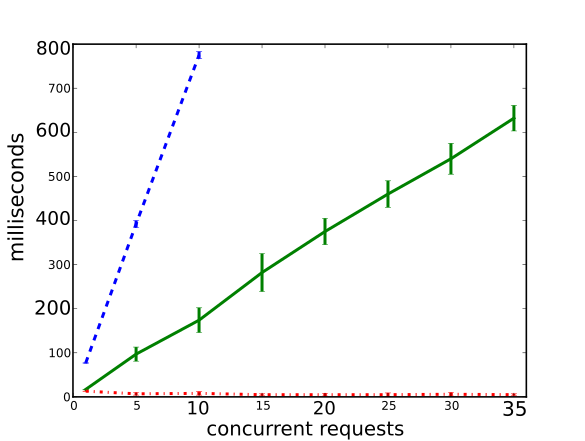
\includegraphics[width=3in]{images/device_comparison.png}
% \label{fig:deviceCompatison}
% \caption{Time measurement comparison among XBee sensors, FoxG20 and a regular computer}
% \end{figure}




\InsertFig{device_comparison}{fig:deviceComparison}{
  Response times measured in different embedded devices
}{
  The dash-dotted line represents the regular computer, the solid line the FoxG20 and the dashed line the XBee.
}{0.7}{}


\begin{table}[htbp]
    \caption{Mean of the measurements taken in different devices with the standard deviation ($\sigma$) in parenthesis.}
    \centering
    \begin{tabular}{|c|c|c|c|}
      \hline
      Concurrent & XBee & FoxG20 & Regular \\
      requests   &  & &  computer \\
      \hline
      1  &  77 (1)	&  17 (0)  &  13 (0) \\
      5  & 392 (8)	&  97 (16) &   7 (3) \\
      10 & 775 (8)	& 174 (28) &   8 (4) \\
      15 &  -	& 282 (43) &   5 (2) \\
      20 &  -	& 375 (30) &   5 (3) \\
      25 &  -	& 460 (30) &   5 (4) \\
      30 &  -	& 540 (35) &   6 (4) \\
      35 &  -	& 632 (29) &   5 (2) \\
      \hline
    \end{tabular}
    \label{tab:timeMeasures}
\end{table}
% añadir uno extra para mencionar los proyectos en los que ha sido usado?
% \input{\pathchapsix/}


\section{Conclusions and further work}

In this paper we have presented our work towards a lightweight flexible Triple Space Computing-based solution called
Otsopack. This framework is specifically designed to adapt to AmI and IoT environments and aims to distribute the
information among different types of nodes in a dynamic way. This forces the design a modular interface, a flexible
networking approach and a simple but yet trustful security layer.

The results show that firstly, the effort required to develop particular features of Otsopack on different platforms is
low, due to its simplicity and the use of standard HTTP capabilities. Secondly, the networking layer shows its ability
to adapt to a wide range of scenarios both in simulation and real environments. Finally, the distributed security schema
allows to automatically expose and share the information managed by the applications so multiple applications that did
not know each other can still interact.

To detail future directions, we aim to implement a notifications system that permits other nodes to know that an event
has occurred. Regarding the security of the information, work is being done to ensure security in certain deployments,
adapting research already done on secure multicast \cite{naranjo2011suite} techniques.



% ----------------------------------------------------------------------

